\chapter{BACKGROUND}

Some scholars found that current Boolean search and filtering techniques cannot satisfy the complexity of candidate-job matching requirement~\cite{malinowski2006matching}. They hope the system can understand the job requirement, determine which requirements are mandatory and which are optional, but preferable. So they moved to use recommender systems technique to address the problem of information overflow. Recommender systems are broadly accepted in
various areas to suggest products, services, and information items to latent customers.


\section{Recommender System}

Job searching, which has been the focus of some commercial job finding web sites and research papers is not a new topic in information retrieval. Usually scholars called them Job Recommender Systems (JRS), because most of them used technologies from recommender systems. Wei et al. classified Recommender Systems into four categories~\cite{wei2007survey}: Collaborative Filtering, Content-based filtering, Knowledge-based and Hybrid approaches. Some of these techniques had been applied into JRS; Zheng et al.~\cite{siting2012job} and AlOtaibi et al.~\cite{al2012survey} summarized the categories of existing online recruiting platforms and listed the advantages and disadvantages of technical approaches in different JRSs. The categories include:

\begin{enumerate}
    \item Content-based Recommendation (CBR). The principle of a content-based recommendation is to suggest items that have similar content information to the corresponding users, like Prospect \cite{singh2010prospect}.

    \item Collaborative Filtering Recommendation (CFR). Collaborative filtering recommendation finds similar  users  who have  the same taste with the target user and recommends items based on what the similar users, like CASPER~\cite{rafter2000personalised}.

    \item Knowledge-based Recommendation (KBR). In the knowledge-based recommendation, rules and patterns obtained from the functional knowledge of how a specific item  meets the requirement of a particular user, are used for recommending items, like  Proactive~\cite{lee2007fighting}.

    \item Hybrid recommender systems combine two or more recommendation techniques to gain better performance, and overcome the drawbacks of any individual one. Usually, collaborative filtering is combined with some other technique in an attempt to avoid the ramp-up problem.

\end{enumerate}

\section{Job Recommender Systems}

Rafter et al. began to use ACF (Automated Collaborative Filtering) in their Job Recommender System, ``CASPER''  \cite{rafter2000personalised}. In the system user profiles are gotten from server logs, that included: revisit data, read time data, and activity data. All these factors were viewed as measure of relevance among users. The system recommend jobs in two steps. First the system find a set of users related to the target user, second the jobs that related users liked will be recommend to the target user. The system use cluster-based Collaborative Filtering strategy. The similarity between users are based on how many jobs they both reviewed, or applied.

The CASPER also allows users to search jobs by a query which is a combination of some fields, like location, salary, skill and so on. The system use such query to find jobs, and the returned jobs will be ranked with above collaborative filtering algorithm. In their paper, they didn't give a detail description on how to detect the related fields they need and how to the transfer semi-structured job description to structured one.

The shortages of Collaborative Filtering: First, since the number of search results is huge, and the results are sorted randomly, the probability of two similar users reviewing the same jobs is low, which causes the sparsity problem of Collaborative Filtering. The authors also noticed the sparseness problem caused by few in users profile, so they try to user cluster-based solution to resolve this problem. Second, because recommended jobs are from others users' search results, since the quality of current searching result are low, the quality of recommendation cannot be high.

F{\"a}rber et al. \cite{farbr2003automated}. presented a recommender system built on a hybrid approach. The system integrated two methods, content-based filtering and collaborative filtering, and tried to overcome the problem of rating data sparsity by leveraging synergies of a combined model, et al. the  latent aspect model. The data they used were synthetic resume. The latent aspect model is shown in Figure~\ref{fig:la}.


\begin{figure}[htbp]
  \centering
  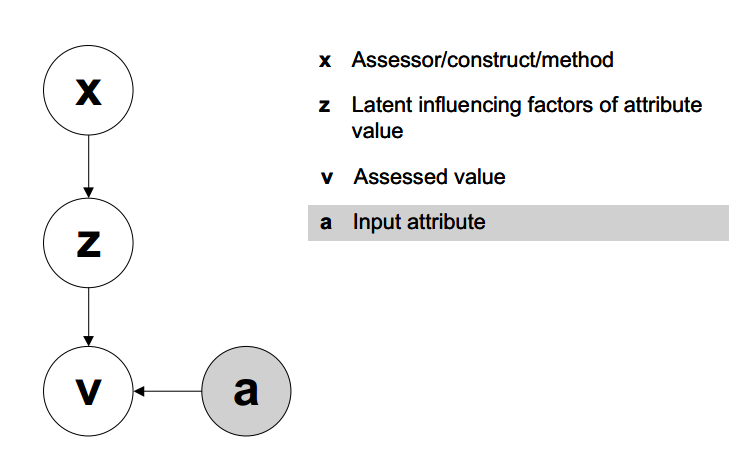
\includegraphics[scale=0.4]{images/la.png}
  \caption{Latent Aspect Model}
  \label{fig:la}
\end{figure}

In Malinowski et al.~\cite{malinowski2006matching} they classified the job recommender systems into two categories,  CV-recommender, which recommends CVs to recruiter, and the job-recommender, which recommends jobs to job seekers. The system collect the users' profile data by asking input their profiles to the web form based interface field by field. The input data collected are:

\begin{enumerate}
    \item  Demographic data (e.g. date of birth, contact information)

    \item  Educational data (e.g. school courses, grades, university, type of degree, intermediate and final university examinations, postgraduate studies)

    \item  Job experience (e.g. name of the company, type of employment, industry group, occupational field)
    \item  Language skills (e.g. language, level of knowledge)
    \item  IT skills (e.g. type of skill, level of knowledge)
    \item  Awards, scholarships, publications, others

\end{enumerate}
The system also asked the users to upload their resumes, but the resumes were only for facilitating the human judgment. In Malinowski's study, the latent aspect model is a statistical model, which needs to be trained before applied to recommendation. The system use the users' search results as the training data to train the model for recommendation, so the system needs a a long time training for each user.


\section{Information Extraction in Job Recommender System}

Big IT companies met the similar problem of information overflow when they received many resumes for one job opening. The recruiter had to screen the all the applications manually, but this task was also tedious and time consuming. For this reason these companies tried to build systems to help screen the resumes.

Amit et al. in IBM presented a system, ``PROSPECT''~\cite{singh2010prospect}, to aid    shortlisting of candidates for jobs. The system uses a r\'esum\'e miner to extract the information from r\'esum\'es, which use a CRF model to segment and label the r\'esum\'es. The CRF model used three kinds of features, they are: Lexicon, Visual, Named Entity, Text, and Conjunction. The paper compared some algorithms to ranked the candidates applicants, such methods include: Okapi BM25, KL, Lucene Scoring, and Lucene Scoring + SkillBoost.

HP also built a system to solve the similar problem, which is introduced in Gonzalez et al.'s paper~\cite{gonzalez2012adaptive}. The system also pays a lot of attention to information extraction. The IE architecture they use is shown in Figure~\ref{fig:hpie}.


\begin{figure}[htbp]
  \centering
  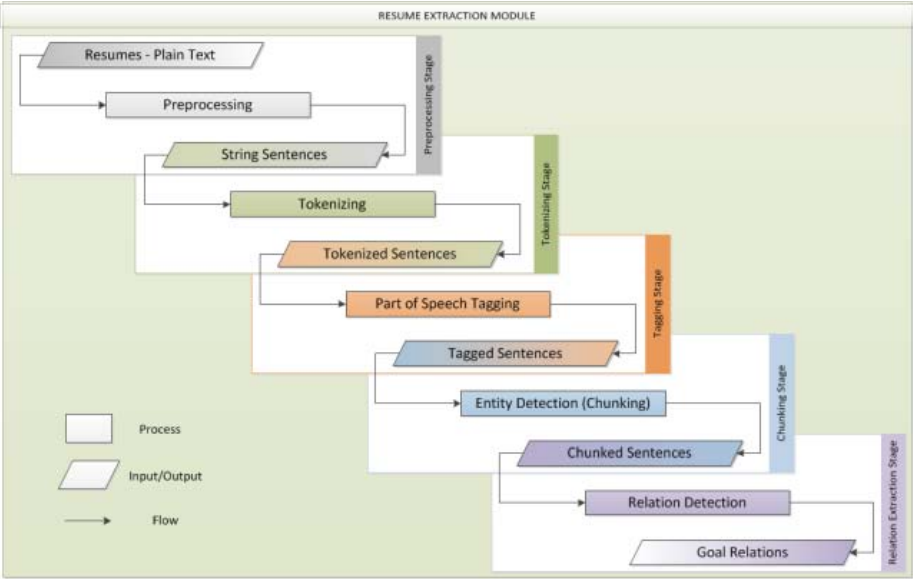
\includegraphics[scale=0.5]{images/hpie.png}
  \caption{IE Framework}
  \label{fig:hpie}
\end{figure}

The dictionaries which were used to tag entities should be updated often since there always new terms appears. So an adaptive learning module is used to achieve two objectives: use semantic data to enhance the information extraction and to discover new terms.

A domain-oriented ontology is used to represent knowledge, inference rules are defined based on the ontology knowledge base. When a detected term found, the system will search in external knowledge base, like DBpedia etc. The r\'esum\'e also be classified to different categories like ``Web Technology'' and ``No Web Technology'' by naive Bayes classifier. The company could allocate appropriate employees to required positions.

The goal of the systems built by IBM and HP is to help the companies to select good applicants. Our system is designed for helping job seekers to find appropriate jobs.  

Yu et al.~\cite{yu2005resume} used a cascaded information extraction (IE) framework to get the detailed information from the job seeker��s r\'esum\'e. In the first stage, the Hidden Markov Modeling (HMM) model is used to segment the r\'esum\'e into consecutive blocks. Based on the result, a SVM model is used to obtain the detailed information in the certain block, the information include: name, address, education etc.

Celik Duygua and Elci Atilla proposed a Ontology-based R��sum�� Parser (ORP) ~\cite{ccelik2013ontology}, which uses ontology to assistant the information extraction process. The system process the r\'esum\'e in following steps: convert the r\'esum\'e files into plain text, separate the text into  some segments, use Ontology Knowledge Base to find the concepts in the sentences, normalize all the terms, at last the system will classify the sentences to get the wanted terms.

But the personal information they retrieved in these works like name and addresses are not the information that the recruiters care about. The recruiters want some information that relate to the job opening, and can help them judge the competence of job applicants.

\section{Matching Algorithms in Job Recommender Systems}

Lu et al.~\cite{lu2013recommender} used latent Semantic Analysis(LSA) to calculate similarities between jobs and candidates, but they only selected two factors ``interest'' and ``education''  to compare candidates. Xing et al.~\cite{yi2007matching} used Structured Relevance Models (SRM) to  match r\'esum\'es and jobs.

Drigas* et al.\cite{drigas2004expert}  presented a expert system to match jobs and job seekers, and recommend unemployed to the positions. The expert system used Neuro-Fuzzy rule to evaluate the matching between user profile and job opening. The system use a relation matrix to represent the fuzzy relation between these specialities. The system need the training data to train that Neuro-fuzzy network. Both r\'esum\'e data and job opening data were manually input into the system.

Daramola et al.\cite{daramola2010fuzzy}  also proposed a fuzzy logic based expert system(FES) tool for online personnel recruitment. In the paper, the authors assumed that the information already be collected. The system use a fuzzy distance metric to rank candidates' profile in the order of their eligibility for the job. The fuzzy hamming distance is given as:
$$ \delta \left ( O,R \right )=\sum_{i=1}^{n}\left | \mu_O(x_i) - \mu_R(x_i)  \right | $$

Yao et al.~\cite{lu2013recommender} also presented a hybrid recommender system which integrated content-based and interaction-based relation. In content-based part, relations between job-job, job-job seeker, and job seeker - job seeker can be identified by their similarity of profiles. There two approaches are used to calculate the similarities: For the structured data, like age gender  etc., the weight sum values will be returned, for the unstructured data like similarity between job and user profile the Latent Semantic Analysis will be used.

There are some problems exist in previous Job Recommender Systems: 
\begin{enumerate}
    \item  Most systems can only process the structured data of r\'esum\'es and job descriptions, but in reality both them are in un-structured formats, like text files or HTML web pages. 

    \item  The systems that have information extraction function are designed for recruiters to select applicants, not for job seekers to select jobs.

    \item  In the systems the information fields to match r\'esum\'es and job descriptions are coarse-grained. To improve the quality of recommendation,  we need to improve the granularity of information fields and matching algorithm.

\end{enumerate}
